\documentclass{article}
\usepackage{amsmath}
\usepackage{amssymb}
\usepackage{graphicx}
\usepackage{hyperref}
\usepackage[version=4]{mhchem}

\title{Example 8}
\date{}

\begin{document}
\maketitle

(AMC) In \(\triangle A B C, D\) is on \(A C\) and \(F\) is on \(B C\). Also \(A B \perp A C, A F \perp\) \(B C\), and \(B D=D C=F C=1\). Find \(A C\).

Solution: \(\sqrt[3]{2}\)\\
Draw \(D G\) so that \(D G \perp B C\) and \(G\) lies on \(B C\). Let \(A C=x\)\\
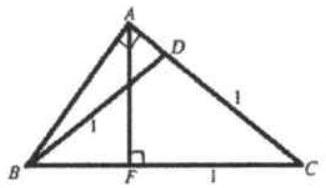
\includegraphics[width=\textwidth]{images/problem_image_1.jpg} and \(G C=y\). Note that \(B C=2 y\), since \(\triangle B C D\) is isosceles.


Since \(\triangle D C G \sim \triangle A C F \sim \triangle B C A\), we obtain the equal ratios: \(\frac{D C}{G C}=\frac{A C}{C F}=\frac{B C}{A C} \quad \Rightarrow \quad \frac{1}{y}=\frac{x}{1}=\frac{2 y}{x}\). Thus \(y=\frac{1}{x}\) and \(y=\frac{x^{2}}{2}\), implying that\\
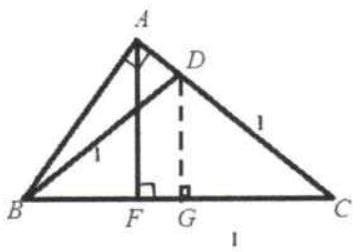
\includegraphics[width=\textwidth]{images/reasoning_image_1.jpg} \(x^{3}=2\), or \(x=\sqrt[3]{2}\).


\end{document}
